\chapter[Fundamentação Teórica]{Fundamentação Teórica}
\label{cha:fundamentacao-teorica}

\section{O que é Teoria dos Jogos?}
\label{sec:o-que-e-teoria-dos-jogos}

Teoria dos jogos é o estudo do comportamento estratégico interdependente\footnote{Estratégia interdependente significa que as ações de uma pessoa interfere no resultado da outra, e vice-versa.}\cite{spaniel_2011}, não apenas o estudo de como vencer ou perder em um jogo, apesar de às vezes esses dois fatos coincidem. Isso faz com que o escopo seja mais abranjente, desde comportamentos no qual as duas pessoas devem cooperar para ganhar, ou as duas tentam se ajudar, ou, por fim, comportamento de duas pessoas que tentam vencer individualmente.

\section{Histórico da Teoria dos Jogos}
\label{sec:historico-da-teoria-dos-jogos}

Pode-se dizer que a análise de jogos é praticada desde o séculco XVIII tendo como evidência uma carta escrita por James Waldegrave ao analisar uma versão curta de um jogo de baralho chamado \emph{le Her} \cite{Prague_severalmilestones}, explicado na seção \ref{subsec:analise-primitiva-do-jogo-le-her}. No século seguinte, Augustin Cournot fez uso da teoria dos jogos para estudos relacionados à política \cite{cournot_1838}. Mais recentemente, em 1913, Ernst Zermelo publica o primeiro teorema matemático da teoria dos jogos \cite{zermelo_1913}.

Dois grandes matemáticos que se interessaram na teoria dos jogos foram Émile Borel e John von Neumann. Nas décadas de 1920 e 1930, Emile Borel publicou três artigos \cite{borel_1921} \cite{borel_1924} \cite{borel_1927} e um livro \cite{borel_1938} sobre jogos estratégicos, introduzindo uma noção abstrada sobre jogo estratégico e estratégia mista. Em 1928, John von Neumann demonstrou que todo jogo finito de soma zero\footnote{Um jogo soma zero é um jogo no qual a vitória de um jogador implica na derrota do outro.} com duas pessoas possui uma solução em estratégias mistas \cite{neumann_1928}. Em 1944, Neumann publicou um trabalho, junto a Oscar Morgenstern \cite{neumann_1944}, e com isso, a teoria dos jogos entrou na área da economia e matemática aplicada.

Outro matemático que contribuiu para a área foi John Forbes Nash Júnior, que publicou quatro artigos importantes para teoria dos jogos não-cooperativos. Dois destes artigos \cite{nash_1950} \cite{nash_1951} provando a existência de um equilíbrio de estratégias mistas para jogos não-cooperativos, denominado \textbf{equilíbrio de Nash}, que será explicado na seção \ref{subsubsec:equilibrio-de-nash}. Nash recebeu o prêmio Nobel em 1994, junto com John Harsanyi e Reinhard Selten, por suas contribuições para a teoria dos jogos.

\section{Conceitos Fundamentais da Teoria dos Jogos}
\label{sec:conceitos-fundamentais-da-teoria-dos-jogos}

Esta seção introduz os conceitos fundamentais da teoria dos jogos, tais como definição de um jogo não cooperativo, formas de representá-lo e teoremas para encontrar soluções.

\subsection{Definição de Jogo Não Cooperativo}
\label{subsec:definicao-de-jogo-nao-cooperativo}

Considerando a definição de um jogo como sendo uma atividade interativa e competitiva no qual os jogadores devem obedecer a um determinado conjunto de regras, então um jogo não cooperativo não permite nenhum tipo de acordo entre os jogadores e o ganho de cada jogador é determinado pelo conjunto de regras \cite{jones_1980}.

\subsection{Estratégia Pura}
\label{subsec:estrategia-pura}

Estratégia pura é um conjunto de escolhas a se fazer para cada momento de decisão possível. Considere o seguinte exemplo retirado do livro de Willian Spaniel \cite{spaniel_2011}: Uma empresa $A$ quer entrar no mercado onde outra empresa $B$ possui o monopólio. Se a empresa $A$ entrar no mercado, a outra pode decidir aceitar ou declarar uma guerra de preços. Considerando que a empresa $A$ só quer entrar no mercado se a empresa $B$ não declarar guerra de preços, e que a guerra de preços não é lucrativa para a empresa $B$, a situação é representada na figura \ref{fig:jogo-do-monopolio}.

\begin{figure}
	\centering
	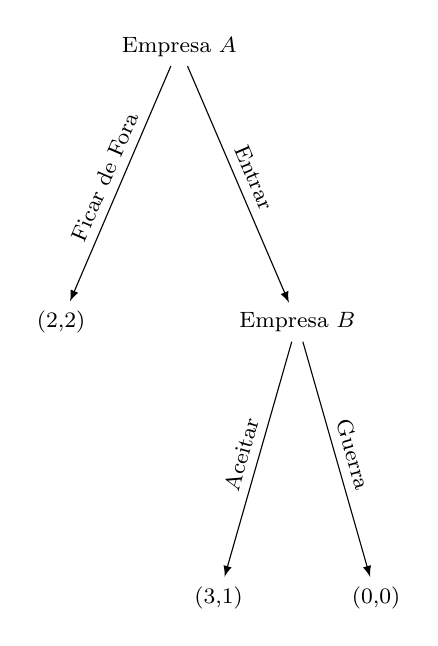
\begin{tikzpicture}
	  [
	    grow                    = down,
	    level distance          = 3.5cm,
	    edge from parent/.style = {draw, -latex},
	    every node/.style       = {font=\footnotesize},
	    sloped,
		level 1/.style			= {sibling distance=3cm},
		level 2/.style			= {sibling distance=2cm}
		]
	  \node {Empresa $A$}
	  	child { node {(2,2)}
	  		edge from parent node [above] {Ficar de Fora} }
	    child { node {Empresa $B$} {
				child { node {(3,1)}
					edge from parent node [above] {Aceitar}
					}
				child { node {(0,0)}
					edge from parent node [above] {Guerra}
					}
				}
			edge from parent node [above] {Entrar}
		};
	\end{tikzpicture}
	\caption{Jogo do monopólio, fonte: \cite{spaniel_2011}}
	\label{fig:jogo-do-monopolio}
\end{figure}

\subsection{Soluções para jogos}
Uma solução de um jogo é uma prescrição ou previsão sobre o resultado do jogo. Há soluções para os jogos que as escolhas dos jogadores são feitas simultaneamente e soluções para os jogos que possuem turnos. Para o primeiro caso, as soluções são encontradas fazendo uso de \textbf{dominância estrita iterada}, enquanto para o segundo caso a solução é encontrada utilizando-se de \textbf{\emph{backward induction}}.

\subsubsection{Dominância estrita}

É dito que uma estratégia é {\bfseries estritamente dominada} para um jogador se esta estratégia gera um ganho maior do que qualquer outra estratégia independente do que o outro jogador fizer. Considera-se que jogadores racionais nunca fazem uso de estratégias estritamente dominadas, pois não há motivos para escolher uma estratégia que sempre será pior em todos os casos. O exemplo do {\bfseries dilema do prisioneiro} demonstra tal conceito.

\subsubsubsection{O Dilema do Prisioneiro}
Formulado por Albert W. Tucker em 1950 \cite{sartini_IIbienaldasbm}, o dilema do prisioneiro é, provavelmente, um dos exemplos mais conhecidos na teoria dos jogos. O propósito de Tucker foi ilustrar a dificuldade de se analisar certos tipos de jogos por razões que ficarão óbvias após o exemplo. Eis a situação: dois suspeitos são presos com suspeita de roubo mas os policiais podem apenas provar que os suspeitos invadiram o local. Precisando da confissão dos criminosos, o policial faz a seguinte proposta
\begin{itemize}
	\tightlist
	\item Se nenhum confessar o roubo, o policial vai prendê-los por intrusão.
	\item Se um confessar e o outro não, o que confessou será liberto e o calado será preso por 12 meses.
	\item Se os dois confessarem, ambos serão presos por 8 meses.
\end{itemize}

Dado essas informações, é possível representá-las no formato {\bfseries matriz de \emph{payoffs}} de acordo com a tabela \ref{tab:dilema-prisioneiro}, onde o ganho do \emph{jogador linha} é representado pelo número à esquerda dentro de uma célula, e o ganho do \emph{jogador coluna} é representado à direita.

\begin{table}[ht]
\centering
\begin{tabular}{|c|c|c|c|}
	\cline{3-4}
	\multicolumn{1}{c}{} &  & \multicolumn{2}{c|}{{\bfseries Coluna}}\tabularnewline
	\cline{3-4}
	\multicolumn{1}{c}{} &  & {\scshape Quieto}\  & {\scshape Confessa}\ \tabularnewline
	\hline
	\multirow{2}{*}{\begin{turn}{90}
	{\bfseries Linha}
	\end{turn}} & \begin{turn}{90}
	{\scshape Quieto}\
	\end{turn} & {\Large(}{\Large -1,}{\Large -1)} & {\Large(}{\Large -12,}{\Large 0)}\tabularnewline
	\cline{2-4}
	 & \begin{turn}{90}
	{\scshape Confessa}\
	\end{turn} & {\Large(}{\Large 0,}{\Large -12)} & {\Large(}{\Large -8,}{\Large -8)}\tabularnewline
	\hline
\end{tabular}
\caption{Dilema do prisioneiro, fonte: \cite{spaniel_2011}}
\label{tab:dilema-prisioneiro}
\end{table}

Considerando que os dois suspeitos querem minimizar seu tempo na cadeia, eles devem confessar à polícia?

Para resolver este jogo é preciso raciocinar como um jogador responderia de acordo com a ação do outro. Supondo que o \emph{jogador coluna} fique \emph{Quieto}, o \emph{jogador linha} pode ficar \emph{Quieto} e ir pra cadeia por 1 mês, sendo representado na tabela \ref{tab:dilema-prisioneiro} pela célula superior esquerda, ou aceitar a proposta do policial e \emph{Confessar} o crime que iriam cometer, sendo representado pela célula inferior esquerda. Como os jogadores querem minimizar seu tempo na prisão, que é representado por um valor negativo, deve-se buscar o maior valor dentre essas duas escolhas, que neste caso é \emph{Confessar} com um ganho de \emph{0}. Observando a outra possibilidade do \emph{jogador coluna}, que seria \emph{Confessar}, o \emph{jogador linha} teria um ganho de \emph{-12} ao ficar \emph{Quieto} e um ganho de \emph{-8} ao \emph{Confessar}. Em ambos os casos, o \emph{jogador linha} terá um melhor ganho ao \emph{Confessar}, e como o jogo é simétrico\footnote{Um jogo é dito simétrico quando as regras são as mesmas para todos os jogadores.} o mesmo raciocínio pode ser feito para o \emph{jogador coluna}.

Essa preferência de \emph{Confessar} a ficar \emph{Quieto} para cada escolha do outro jogador (\emph{Quieto} ou \emph{Confessar}) é dito que \emph{Confessar} é estritamente dominante.

\subsubsection{Eliminação iterada de estratégias estritamente dominadas}

Eliminação por dominância estrita iterada, como o próprio nome já diz, é um processo iterado no qual estratégias são eliminadas por serem dominadas estritamente \cite{spaniel_2011}. Se uma estratégia for estritamente dominada, elimine-a imediatamente, não importando a ordem da eliminação. Se ao final do processo sobrar apenas uma única célula, este resultado será alcançado começando a eliminação por qualquer estratégia estritamente dominada. Considere a tabela \ref{tab:dominancia-estrita-iterada}.

\begin{table}[ht]
\centering
\begin{tabular}{|c|c|c|c|c|}
\cline{3-5}
\multicolumn{1}{c}{} &  & \multicolumn{3}{c|}{\textbf{Jogador Coluna}}\tabularnewline
\cline{3-5}
\multicolumn{1}{c}{} &  & \textsc{Esquerda} & \textsc{Centro} & \textsc{Direita}\tabularnewline
\hline
\multirow{3}{*}{\begin{turn}{90}
\textbf{Jogador Linha}
\end{turn}} & \begin{turn}{90}
\textsc{Cima}
\end{turn} & {\Large(13,3)} & {\Large(1,4)} & {\Large(7,3)} \tabularnewline
\cline{2-5}
 & \begin{turn}{90}
\textsc{Meio}
\end{turn} & {\Large(4,1)} & {\Large(3,3)} & {\Large(6,2)} \tabularnewline
\cline{2-5}
 & \begin{turn}{90}
\textsc{Baixo}
\end{turn} &  {\Large(-1,9)} & {\Large(2,8)} & {\Large(8,-1)} \tabularnewline
\hline
\end{tabular}
\caption{Exemplo de dominância estrita iterada, fonte: \cite{spaniel_2011}}
\label{tab:dominancia-estrita-iterada}
\end{table}

Na tabela \ref{tab:dominancia-estrita-iterada}, o \emph{jogador linha} tem três estratégias \emph{cima}, \emph{meio} e \emph{baixo}, enquanto o \emph{jogador coluna} possui as estratégias \emph{esquerda}, \emph{centro} e \emph{direita}, gerando um total de 9 resultados.
Observando as estratégias do \emph{jogador linha}, não é possível fazer nenhuma dominância estrita, pois o \emph{jogador linha} possui uma preferência diferente de suas próprias estratégias para cada estratégia do \emph{jogador coluna}. No caso da estratégia \emph{esquerda}, a melhor estratégia para o \emph{jogador linha} é \emph{cima}, assim como \emph{centro} e \emph{meio}, e \emph{direita} e \emph{baixo}.

Porém, observando as estratégias \emph{centro} e \emph{direita}, é possível eliminar a segunda estratégia por dominância estrita, pois, para o \emph{jogador coluna}, todos os ganhos da estratégia \emph{centro} são melhores do que os ganhos da estratégia \emph{direita}. Com a eliminação da estratégia \emph{direita}, é possível eliminar a estratégia \emph{baixo}, que é estritamente dominada pela estratégia \emph{meio} para o \emph{jogador linha}. Com essas duas eliminações, é possível eliminar as estratégias \emph{esquerda}, pois, para o jogador \emph{jogador coluna}, é estritamente dominada pela estratégia \emph{centro}, e por fim, para o jogador \emph{jogador linha}, a estratégia \emph{cima} é estritamente dominada pela estratégia \emph{meio}.

No final da eliminação iterada de estratégias estritamente dominadas. sobra apenas uma única célula da tabela \ref{tab:dominancia-estrita-iterada}, como demonstrado na tabela \ref{tab:final-dominancia-estrita-iterada}, e é chamado de \textbf{equilíbrio de estratégia dominante}.

\begin{table}[ht]
\centering
\begin{tabular}{|c|c|}
\cline{2-2}
\multicolumn{1}{c|}{} & {\scshape Centro} \tabularnewline
\hline
\begin{turn}{90}
{\scshape Meio}
\end{turn} &  {\Large(}{\Large 3,}{\Large 3)}\tabularnewline
\hline
\end{tabular}
\caption{Final do exemplo de dominância estrita iterada, fonte: \cite{spaniel_2011}}
\label{tab:final-dominancia-estrita-iterada}
\end{table}

\subsubsection{Estratégia Pura}

Considere a situação a seguir: Dois caçadores devem decidir o que caçar no dia e levar o equipamento apropriado. Eles sabem que, no local de caça, existem duas lebres, que valem uma unidade de carne cada, e um veado, que vale seis unidades de carne. O veado vale mais carne dividindo para cada um do que a soma das duas lebres, mas é preciso o auxílio do outro caçador para caçar um veado, enquanto as lebres podem ser caçadas sem nenhuma ajuda \cite{spaniel_2011}. Estas informações são condensadas na tabela \ref{tab:caca-ao-viado}.

\begin{table}[ht]
\centering
\begin{tabular}{|c|c|c|c|}
	\cline{3-4}
	\multicolumn{1}{c}{} &  & \multicolumn{2}{c|}{{\bfseries Coluna}}\tabularnewline
	\cline{3-4}
	\multicolumn{1}{c}{} &  & {\scshape Veado}\  & {\scshape Lebre}\ \tabularnewline
	\hline
	\multirow{2}{*}{\begin{turn}{90}
	{\bfseries Linha}
	\end{turn}} & \begin{turn}{90}
	{\scshape Veado}\
	\end{turn} & {\Large(3,3)} & {\Large(0,2)}\tabularnewline
	\cline{2-4}
	 & \begin{turn}{90}
	{\scshape Lebre}\
	\end{turn} & {\Large(2,0)} & {\Large(1,1)}\tabularnewline
	\hline
\end{tabular}
\caption{Caça ao Veado, fonte: \cite{spaniel_2011}}
\label{tab:caca-ao-viado}
\end{table}




\subsubsection{Teorema Minimax}
\label{subsubsec:teorema-minimax}

\subsubsection{Equilíbrio de Nash}
\label{subsubsec:equilibrio-de-nash}



\subsection{Análise primitiva do jogo \emph{le Her}}
\label{subsec:analise-primitiva-do-jogo-le-her}

O objetivo do jogo \emph{le Her} é terminar o jogo com a carta mais alta, sendo que o baralho é contado de Ás ($A$) à Rei ($K$). Essa versão reduzida podia ser jogada apenas com dois jogadores, um deles chamado \emph{dealer} e outro \emph{receiver}. O \emph{dealer} embaralha as cartas e distribui uma carta para o \emph{receiver} e uma para si. O \emph{receiver} tem a escolha de manter sua carta ou trocá-la com o \emph{dealer}, e em seguida o \emph{dealer} tem a mesma opção de manter ou de trocar sua carta com uma carta nova do baralho. A única regra que impede a troca é o caso da carta recebida ser um Rei ($K$), neste caso a troca deve ser desfeita e o jogador mantém sua carta original.

%Vários artigos apontam


\subsection{Representação de um Jogo}
\label{subsec:representacao-de-um-jogo}

Há duas formas de representar um jogo de uma maneira que seja possível analisá-lo em seguida, a \textbf{forma extensiva} e a \textbf{forma normal}. A forma extensiva faz uso de uma estrutura de árvore, onde os nós representam estados do jogo e as arestas representam as jogadas possíveis a partir daquele estado. Dado um jogo $\Gamma$, não cooperativo com \emph{n} jogadores tem-se:


\section{O Jogo \emph{Big Points}}
\subsection{Conceito do Jogo}
\emph{Big Points} é um jogo abstrato e estratégico com uma mecânica de colecionar peças. São cinco peões de cores distintas, que podem ser usadas por qualquer jogador, para percorrer um caminho de discos coloridos até chegar ao pódio. Durante o percurso, os jogadores coletam alguns destes discos. A pontuação de cada jogador é determinada a partir da ordem de chegada dos peões ao pódio e a quantidade de discos adquiridos de cada cor. Ganha o jogador com a maior pontuação.

\subsection{Regras do Jogo}
O jogo \emph{Big Points} pode ser jogado de dois a cinco jogadores. No seu turno, o jogador escolhe qualquer um dos cinco peões, que possuem cores distintas, e o move para cima do próximo disco de sua mesma cor. Em seguida, o jogador deve pegar o próximo disco disponível\footnote{É dito indisponível aqueles discos que já foram pegos por algum jogador ou que possuem um peão em cima.} à frente ou atrás deste peão. Caso não haja discos atrás (à frente) do peão, o jogador deve pegar o disco que está à frente (atrás). Caso o jogador já possua um disco preto no começo do turno, tal jogador pode escolher descartá-lo para realizar um segundo movimento. Este movimento pode ser com qualquer cor de peão como uma jogada normal, mas dessa vez o movimento pode ser feito para trás.
